%!TEX root=main.tex
\section{Diagnosing a Trend} \label{sec:data}
Before the LHC became operational in 2010, there were strong expectations for new physics and accordingly there existed a whole landscape of BSM models. 
The Higgs boson was discovered in 2012, but none of the searches for new physics turned up anything significant enough to indicate BSM physics.
Analyses are increasingly constraining the existing BSM models, and designing experimental searches based on model-specific predictions seems less and less fruitful. 
Physicists are thus increasingly turning to alternative methods for searching for new physics, they are using simplified models and so-called model-independent approaches, among them EFTs.
This trend away from model-guided searches and towards model-independent approaches can already be documented with simple bibliographic means.
Figure~1 shows the results of a keyword search that compares the most popular BSM model, viz. supersymmetry, with the effective field theory approach. 
The search was conducted on the popular physics preprint archive, archive.org.
Specifically, it was conducted on the archives most relevant to high-energy physics, the phenomenology and experimental archives HEP-PH and HEP-EX. 
We have shown in previous publications that such keyword searches provide a good first look at the dynamics of particle physics models and that the corresponding trends can be confirmed by expert interviews.\footnote{For a full description of the methods used, see [reference omitted].}

The main reason such figures provide a reasonable first look is that the mentioned preprint archives are the main scientific venue for particle physicists.
ArXiv.org features an automatic keyword tagging system.
This system provides us with a simple method of gauging some of the trends in particle physics by seeing how the numbers of papers with different keywords change over time.\footnote{The keywords used were the following. For EFT: find k "effective field theory" and (primarch "hep-ph" or primarch "hep-ex"). For SUSY: find k "supersymm*" or k "minimal supersymm*" or k "MSSM" and (primarch "hep-ph" or primarch "hep-ex").} 
\begin{figure}[ht] \label{lineplot}
	\begin{center}
	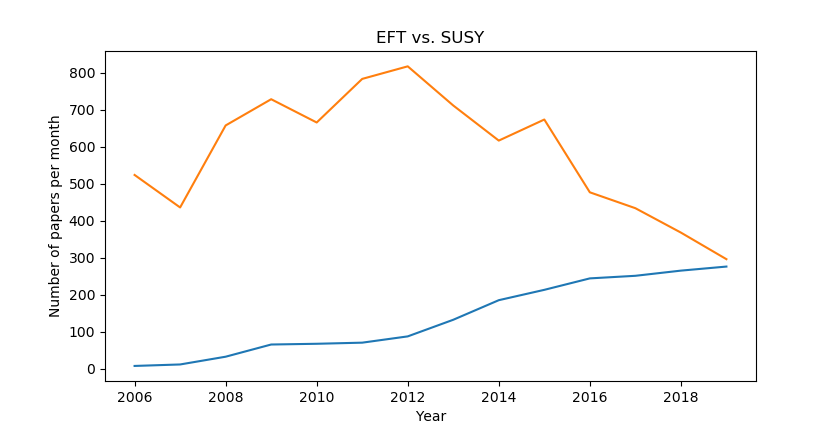
\includegraphics[scale=0.7]{eftsusy2609}
	\caption{Popularity of effective field theories against supersymmetry by number of papers per year on HEP-PH since 2006}
	\end{center}
\end{figure}
\MKnote{I will add proper labels and try to narrow the search in order to be more meaningful.}
We take these searches to indicate that there is a strong trend in particle physics that is worth investigating philosophically.
We also take this to indicate that there is a real distinction between the model-based and model-independent approaches. 
Part of our aim in the paper is to characterise this distinction and see how, or to what degree, the approach is independent from models and how one should understand this in the context of the contemporary debates on the nature of models.
